%  LaTeX support: latex@mdpi.com 
%  For support, please attach all files needed for compiling as well as the log file, and specify your operating system, LaTeX version, and LaTeX editor.

%=================================================================
\documentclass[journal,article,submit,pdftex,moreauthors]{Definitions/mdpi} 
%\documentclass[preprints,article,submit,pdftex,moreauthors]{Definitions/mdpi} 
% For posting an early version of this manuscript as a preprint, you may use "preprints" as the journal. Changing "submit" to "accept" before posting will remove line numbers.

%--------------------
% Class Options:
%--------------------
%----------
% journal
%----------
% Choose between the following MDPI journals:
% accountaudit, acoustics, actuators, addictions, adhesives, adolescents, aerobiology, aerospace, agriculture, agriengineering, agrochemicals, agronomy, ai, aichem, aieng, aimater, aimed, aipa, air, aisens, algorithms, allergies, alloys, amh, analog, analytica, analytics, anatomia, anesthres, animals, antibiotics, antibodies, antioxidants, applbiosci, appliedchem, appliedmath, appliedphys, applmech, applmicrobiol, applnano, applsci, aquacj, architecture, arm, arthropoda, asc, asi, astronautics, astronomy, atmosphere, atoms, audiolres, automation, axioms, bacteria, batteries, bdcc, beverages, biochem, bioengineering, biologics, biology, biomass, biomechanics, biomed, biomedicines, biomedinformatics, biomimetics, biomolecules, biophysica, bioresourbioprod, biosensors, biosphere, biotech, birds, blockchains, bloods, blsf, brainsci, breath, buildings, cancers, carbon, cardio, cardiogenetics, cardiovascmed, catalysts, cells, ceramics, challenges, chemengineering, chemistry, chemosensors, chemproc, children, chips, cimb, civileng, cleantechnol, climate, clinbioenerg, clinpract, clockssleep, cmd, cmtr, coasts, coatings, colloids, colorants, commodities, complexities, complications, compounds, computation, computers, condensedmatter, conservation, constrmater, cosmetics, covid, crops, cryo, cryptography, crystals, csmf, ctn, culture, curroncol, cyber, dairy, data, ddc, dentistry, dermato, dermatopathology, designs, devices, dhi, diabetology, diagnostics, dietetics, digital, disabilities, diseases, diversity, dna, drones, dynamics, earth, ebj, ecm, ecologies, edm, eesp, electricity, electrochem, electronicmat, electronics, encyclopedia, endocrines, energies, eng, engproc, entomology, entropy, environments, environremediat, epidemiologia, epigenomes, esa, est, fermentation, fibers, fintech, fire, fishes, fluids, foods, forecasting, forensicsci, forests, fossstud, foundations, fractalfract, fuels, future, futureinternet, futurepharmacol, futurephys, futuretransp, galaxies, gases, gastroent, gastrointestdisord, gastronomy, gels, genes, geographies, geohazards, geomatics, geometry, geosciences, geotechnics, geriatrics, germs, glacies, grasses, green, greenhealth, gucdd, hardware, hazardousmatters, healthcare, hearts, hemato, hematolrep, hep, heritage, higheredu, highthroughput, horticulturae, hospitals, hydrobiology, hydrogen, hydrology, hydropower, hygiene, idr, iic, ijem, ijerph, ijgi, ijmd, ijms, ijns, ijom, ijpb, ijt, ijtm, ijtpp, ime, immuno, informatics, information, infrastructures, inorganics, insects, instruments, inventions, iot, j, jaestheticmed, jal, jcdd, jcm, jcp, jcrm, jcs, jcto, jdad, jdb, jdream, jemr, jeta, jfb, jfmk, jgbg, jgg, jimaging, jlpea, jmahp, jmmp, jmms, jmp, jmse, jne, jnt, jof, joi, joitmc, joma, jop, joptm, jor, jox, jpbi, jphytomed, jpm, jsan, jtaer, jvd, jzbg, kidneydial, kinasesphosphatases, knowledge, labmed, laboratories, lae, land, life, lights, limnolrev, lipidology, liquids, livers, logics, logistics, lubricants, lymphatics, machines, macromol, magnetism, magnetochemistry, make, marinedrugs, materials, materproc, mathematics, mca, measurements, medicina, medicines, medsci, membranes, merits, metabolites, metals, meteorology, methane, metrics, metrology, micro, microarrays, microbiolres, microelectronics, micromachines, microorganisms, microplastics, microwave, minerals, mining, mmphys, modelling, molbank, molecules, mps, msf, mti, multimedia, muscles, nanoenergyadv, nanomanufacturing, nanomaterials, ncrna, ndt, network, neuroglia, neuroimaging, neurolint, neurosci, nitrogen, notspecified, nursrep, nutraceuticals, nutrients, obesities, occuphealth, oceans, ohbm, onco, optics, oral, organics, organoids, osteology, oxygen, pandemics, parasites, parasitologia, particles, pathogens, pathophysiology, pediatrrep, pets, pharmaceuticals, pharmaceutics, pharmacoepidemiology, pharmacy, philosophies, photochem, photonics, phycology, physchem, physics, physiologia, plants, plasma, platforms, pollutants, polymers, polysaccharides, populations, poultry, powders, precipitation, precisoncol, preprints, proceedings, processes, prosthesis, proteomes, psf, psychiatryint, psychoactives, purification, quantumrep, quaternary, qubs, radiation, rdt, reactions, realestate, receptors, recycling, regeneration, remotesensing, reports, reprodmed, resources, rheumato, rjpm, robotics, rsee, ruminants, safety, sci, scipharm, sclerosis, seeds, sensors, separations, sexes, shi, signals, sinusitis, siuj, skins, smartcities, sna, societies, software, soilsystems, solar, solids, spectroscj, sports, standards, stats, std, stratsediment, stresses, surfaces, surgeries, suschem, sustainability, symmetry, synbio, systems, tae, targets, taxonomy, technologies, telecom, test, textiles, thalassrep, therapeutics, thermo, timespace, tomography, toxics, toxins, tph, transplantology, transportation, traumacare, traumas, tri, tropicalmed, universe, urbansci, uro, vaccines, vehicles, venereology, vetsci, vibration, virtualworlds, viruses, vision, waste, water, welding, wem, wevj, wild, wind, women, world, zoonoticdis

%---------
% article
%---------
% The default type of manuscript is "article", but can be replaced by: 
% abstract, addendum, article, benchmark, book, bookreview, briefcommunication, briefreport, casereport, changes, clinicopathologicalchallenge, comment, commentary, communication, conceptpaper, conferenceproceedings, correction, conferencereport, creative, datadescriptor, discussion, entry, expressionofconcern, extendedabstract, editorial, essay, erratum, fieldguide, hypothesis, interestingimages, letter, meetingreport, monograph, newbookreceived, obituary, opinion, proceedingpaper, projectreport, reply, retraction, review, perspective, protocol, shortnote, studyprotocol, supfile, systematicreview, technicalnote, viewpoint, guidelines, registeredreport, tutorial,  giantsinurology, urologyaroundtheworld
% supfile = supplementary materials

%----------
% submit
%----------
% The class option "submit" will be changed to "accept" by the Editorial Office when the paper is accepted. This will only make changes to the frontpage (e.g., the logo of the journal will get visible), the headings, and the copyright information. Also, line numbering will be removed. Journal info and pagination for accepted papers will also be assigned by the Editorial Office.

%------------------
% moreauthors
%------------------
% If there is only one author the class option oneauthor should be used. Otherwise use the class option moreauthors.

%---------
% pdftex
%---------
% The option pdftex is for use with pdfLaTeX. Remove "pdftex" for (1) compiling with LaTeX & dvi2pdf (if eps figures are used) or for (2) compiling with XeLaTeX.

%=================================================================
% MDPI internal commands - do not modify
\firstpage{1} 
\makeatletter 
\setcounter{page}{\@firstpage} 
\makeatother
\pubvolume{1}
\issuenum{1}
\articlenumber{0}
\pubyear{2026}
\copyrightyear{2026}
%\externaleditor{Firstname Lastname} % More than 1 editor, please add `` and '' before the last editor name
\datereceived{ } 
\daterevised{ } % Comment out if no revised date
\dateaccepted{ } 
\datepublished{ } 
%\datecorrected{} % For corrected papers: "Corrected: XXX" date in the original paper.
%\dateretracted{} % For retracted papers: "Retracted: XXX" date in the original paper.
%\doinum{} % Used for some special journals, like molbank
%\pdfoutput=1 % Uncommented for upload to arXiv.org
%\CorrStatement{yes}  % For updates
%\longauthorlist{yes} % For many authors that exceed the left citation part
%\IsAssociation{yes} % For association journals

%=================================================================
% Add packages and commands here. The following packages are loaded in our class file: fontenc, inputenc, calc, indentfirst, fancyhdr, graphicx, epstopdf, lastpage, ifthen, float, amsmath, amssymb, lineno, setspace, enumitem, mathpazo, booktabs, titlesec, etoolbox, tabto, xcolor, colortbl, soul, multirow, microtype, tikz, totcount, changepage, attrib, upgreek, array, tabularx, pbox, ragged2e, tocloft, marginnote, marginfix, enotez, amsthm, natbib, hyperref, cleveref, scrextend, url, geometry, newfloat, caption, draftwatermark, seqsplit
% cleveref: load \crefname definitions after \begin{document}

%=================================================================
% Please use the following mathematics environments: Theorem, Lemma, Corollary, Proposition, Characterization, Property, Problem, Example, ExamplesandDefinitions, Hypothesis, Remark, Definition, Notation, Assumption
%% For proofs, please use the proof environment (the amsthm package is loaded by the MDPI class).

%=================================================================
% Full title of the paper (Capitalized)
\Title{Hybrid Model for Nontuberculous Mycobacteria Identification:
	NTM-Images Dataset}

% Author Orchid ID: enter ID or remove command
\newcommand{\orcidauthorA}{0000-0000-0000-000X} % Add \orcidA{} behind the author's name
%\newcommand{\orcidauthorB}{0000-0000-0000-000X} % Add \orcidB{} behind the author's name

% Authors, for the paper (add full first names)
\Author{Kazi Saikul Islam Tibro $^{1}$, Monsurul Hoque Akib $^{2}$, Soyoda Meenmoy $^{3}$ Mehejabin Khan Juju $^{4,}$*}

%\longauthorlist{yes}

% MDPI internal command: Authors, for metadata in PDF
\AuthorNames{Kazi Saikul Islam Tibro, Monsurul Hoque Akib, Soyoda Meenmoy and Mehejabin Khan Juju}

% Affiliations / Addresses (Add [1] after \address if there is only one affiliation.)
\address{%
$^{1}$ \quad Department of Computer Science and Engineering, East West University, Dhaka, Bangladesh \\
$^{2}$ \quad Affiliation ; e-mail@e-mail.com}

% Contact information of the corresponding author
\corres{Correspondence: e-mail@e-mail.com; }

% Current address and/or shared authorship
%\firstnote{Current address: Affiliation.}  
% Current address should not be the same as any items in the Affiliation section.

%\secondnote{These authors contributed equally to this work.}
% The commands \thirdnote{} till \eighthnote{} are available for further notes.

%\simplesumm{} % Simple summary

%\conference{} % An extended version of a conference paper

% Abstract (Do not insert blank lines, i.e. \\) 
\abstract{The risk posed to immunocompromised patients by nontuberculous mycobacteria (NTM) as 
	waterborne pathogens will be significant due to their difficulties in visual identification when 
	grown on selective media, because of their morphological similarities to each other. The current 
	methods for identifying NTM are traditional laboratory methods that require anywhere from 2 to 
	6 weeks to produce results and laboratory facilities with very expensive molecular equipment. 
	This study presents the development of an automated image classification system that can 
	successfully classify NTM species based on images of their colonies from NTM Elite agar 
	media. \textbf{Methods:} To extract high-level information, we utilized three pre-trained Convolutional 
	Neural Networks (ResNet50, EfficientNetB3, DenseNet121), and merged these models' features 
	with 34 handcrafted computer vision features that reflected color statistics, GLCM texture, edge 
	density, colony morphology, and Local Binary Patterns (LBP), resulting in a hybrid feature 
	vector that consisted of 4,642 dimensions. Using this combined feature vector as input, we 
	trained a weighted ensemble of five classifiers (XGBoost, Random Forest, Logistic Regression, 
	Support Vector Machine, and a Neural Network) on 561 augmented training images and 
	evaluated it on 92 original images from the public NTM-Images database. \textbf{Results:} The weighted 
	ensemble model was 88.89\% correct, replicating the best performing single model (Neural 
	Network = 90.28\%) while still having considerably more robustness. The Gordonae\_Group, 
	which consists of merged species M. gordonae and M. paragordonae that share 99.0\%  16S RNA 
	sequence identity, achieved 100\% recall.Evaluation of the success of handling phylogenetically 
	similar species. While M. chelonae was the lowest recall (61.5\%) indicating continued 
	morphological variability within both species. Ablation analyses demonstrated that the use of 
	handcrafted features improved model performance by an additional 2.78\% compared to using 
	only deep feature models. \textbf{Conclusion:} The hybrid feature fusion technique along with an ensemble learning approach 
	provides a practical (rapid; cost-effective; and non-invasive) alternative to NTM species 
	identification outside of laboratory settings that will have potential applications for microbiology 
	laboratories and limited resource environments. }

% Keywords
\keyword{Nontuberculous Mycobacteria; NTM-Images dataset; Hybrid features; Ensemble learning; CNN feature extraction; Handcrafted features; Medical image classification; Phylogenetic similarity. }  
% The fields PACS, MSC, and JEL may be left empty or commented out if not applicable
%\PACS{J0101}
%\MSC{}
%\JEL{}

%%%%%%%%%%%%%%%%%%%%%%%%%%%%%%%%%%%%%%%%%%
% Only for the journal Diversity
%\LSID{\url{http://}}

%%%%%%%%%%%%%%%%%%%%%%%%%%%%%%%%%%%%%%%%%%
% Only for the journal Applied Sciences
%\featuredapplication{Authors are encouraged to provide a concise description of the specific application or a potential application of the work. This section is not mandatory.}
%%%%%%%%%%%%%%%%%%%%%%%%%%%%%%%%%%%%%%%%%%

%%%%%%%%%%%%%%%%%%%%%%%%%%%%%%%%%%%%%%%%%%
% Only for the journal Data
%\dataset{DOI number or link to the deposited data set if the data set is published separately. If the data set shall be published as a supplement to this paper, this field will be filled by the journal editors. In this case, please submit the data set as a supplement.}
%\datasetlicense{License under which the data set is made available (CC0, CC-BY, CC-BY-SA, CC-BY-NC, etc.)}

%%%%%%%%%%%%%%%%%%%%%%%%%%%%%%%%%%%%%%%%%%
% Only for the journal BioTech, Fishes, Neuroimaging and Toxins
%\keycontribution{The breakthroughs or highlights of the manuscript. Authors can write one or two sentences to describe the most important part of the paper.}

%%%%%%%%%%%%%%%%%%%%%%%%%%%%%%%%%%%%%%%%%%
% Only for the journal Encyclopedia
%\encyclopediadef{For entry manuscripts only: please provide a brief overview of the entry title instead of an abstract.}

%%%%%%%%%%%%%%%%%%%%%%%%%%%%%%%%%%%%%%%%%%
% Different journals have different requirements. Please check the specific journal guidelines in the "Instructions for Authors" on the journal's official website.
%\addhighlights{yes}
%\renewcommand{\addhighlights}{%
%
%\noindent The goal is to increase the discoverability and readability of the article via search engines and other scholars. Highlights should not be a copy of the abstract, but a simple text allowing the reader to quickly and simplified find out what the article is about and what can be cited from it. Each of these parts should be devoted up to 2~bullet points.\vspace{3pt}\\
%\textbf{What are the main findings?}
% \begin{itemize}[labelsep=2.5mm,topsep=-3pt]
% \item First bullet.
% \item Second bullet.
% \end{itemize}\vspace{3pt}
%\textbf{What are the implications of the main findings?}
% \begin{itemize}[labelsep=2.5mm,topsep=-3pt]
% \item First bullet.
% \item Second bullet.
% \end{itemize}
%}

%%%%%%%%%%%%%%%%%%%%%%%%%%%%%%%%%%%%%%%%%%
\begin{document}

%%%%%%%%%%%%%%%%%%%%%%%%%%%%%%%%%%%%%%%%%%
%\setcounter{section}{-1} %% Remove this when starting to work on the template.%
\newpage
\section{Introduction}

Nontuberculous mycobacteria are a group of tiny living things that are found in water and soil all around us. These Nontuberculous mycobacteria are not like the bacteria that cause tuberculosis they do not usually spread from person to person. Instead people get infected with mycobacteria through things they breathe in or come into contact with in water systems especially in hospitals \cite{falkinham2021} \cite{griffith2007}. More and more people are getting sick with lung diseases caused by mycobacteria with about 1 to 2 people out of every 100,000 getting sick in North America and Europe \cite{prevots2015}. They can also cause infections, in the lymph nodes, skin and soft tissues and even spread to the whole body in people who have very weak immune systems \cite{falkinham2021} \cite{griffith2007}. Traditional identification of mycobacteria or NTM relies on a combination of methods. These methods include culture-based and molecular methods and mass spectrometry methods. Culture on media like Middlebrook 7H11 and NTM Elite agar is the gold standard for diagnosis. This process depends on interpretation which can delay diagnosis and reduce clinical efficiency as shown in \cite{griffith2007}, \cite{biomerieux2023} and \cite{crowley2008}. They are time-consuming and often produce results due to variability among nontuberculous mycobacteria or NTM species as shown in \cite{griffith2007}. However they require equipment and trained personnel. They take 24 to 72 hours to deliver results. It is difficult to distinguish related nontuberculous mycobacteria or NTM species due to high genetic similarity as shown in \cite{griffith2007} and \cite{turenne2018}. However it is expensive and limited by database coverage for nontuberculous mycobacteria or NTM species. Sample preparation is complex due, to the structure of the mycobacterial cell wall as shown in \cite{griffith2007}. They have genes and grow in similar ways \cite{biomerieux2023} \cite{crowley2008} \cite{turenne2018}. We need ways to automatically identify NTM infections \cite{falkinham2021} \cite{griffith2007}. We are also using learning and convolutional neural networks to classify medical and microbiological images \cite{litjens2017}; \cite{pan2022}; \cite{dietterich2000}; \cite{kumar2017}; \cite{haralick1973}; \cite{ojala2002}; \cite{esteva2017}; \cite{crowley2008}; \cite{he2016}; \cite{tan2019}; \cite{huang2017}. Machine learning and deep learning are options for telling apart NTM species that look and are genetically similar where lab methods do not work well \cite{crowley2008}; \cite{mendeley2025}.


%%%%%%%%%%%%%%%%%%%%%%%%%%%%%%%%%%%%%%%%%%
\section{Related Work}

The ecology and clinical importance of mycobacteria or NTM have been widely studied, particularly because of their presence in environmental sources such as water and soil and their role as opportunistic pathogens that is NTM. NTM are highly resistant to disinfectants. Commonly affect immunocompromised individuals as stated in reference \cite{falkinham2021}.The global prevalence of NTM infections has been increasing, with risk factors including age, pre-existing lung disease and geographic variation in species distribution as mentioned in reference \cite{prevots2015}.Clinical guidelines emphasize that identification of NTM species, such as NTM is essential for effective treatment although current diagnostic procedures are complex and time-consuming as explained in reference \cite{griffith2007}. 

Advances in culture media such as NTM Elite agar, have improved detection speed and contamination control but species-level identification remains challenging due to morphological similarities as discussed in reference \cite{biomerieux2023}.This challenge is further highlighted by similar species such as Mycobacterium gordonae and Mycobacterium paragordonae, which share approximately 99\% 16S rRNA sequence similarity making them difficult to distinguish using conventional methods as stated in reference \cite{turenne2018}.Recent developments in intelligence particularly deep learning have significantly improved medical image analysis, including the analysis of images related to NTM. Convolutional Neural Networks or CNNs have demonstrated performance across various domains, including radiology, pathology and dermatology as highlighted in a comprehensive survey of over 300 studies reference \cite{litjens2017}.

In the context of microbiology deep learning has been applied to classify species, including NTM from microscopy images achieving promising accuracy although limitations remain due to small and non-public datasets as mentioned in reference \cite{smith2023}.Comparative studies of CNN architectures have shown that ensemble approaches improve robustness and classification performance with models such as DenseNet121 demonstrating individual performance as explained in reference \cite{pan2022}.The theoretical foundation of learning explains these improvements through variance reduction, avoidance of local optima and increased representational capacity as discussed in reference \cite{dietterich2000}.
 
Empirical evidence further supports this as ensemble models have outperformed CNNs in medical imaging tasks such as pneumonia detection reference \cite{kumar2017}. In addition to learning traditional image processing techniques continue to play an important role in feature extraction including the analysis of images related to NTM. Texture-based methods, such as Gray-Level Co- Matrix or GLCM features and Local Binary Patterns or LBP have proven effective in capturing structural patterns in images as stated in reference \cite{haralick1973, ojala2002}.
 
These techniques have been successfully applied to colony characterization, where texture features help distinguish visually similar species, including NTM as explained in reference \cite{johnson2022}. More recent studies have shown that combining deep learning features with features leads to improved classification performance demonstrating the effectiveness of hybrid approaches as mentioned in reference \cite{zhang2024}.
 
Similar success has been observed in domains, such as plant disease detection using transfer learning reference \cite{chen2020} and skin cancer classification achieving dermatologist-level accuracy reference \cite{esteva2017}. Deep learning has also been applied to tuberculosis detection further highlighting its potential in disease diagnosis including the diagnosis of NTM infections as stated in reference \cite{lopez2017}.
 
Early work in automated colony identification using texture analysis laid the foundation for these modern approaches as explained in reference \cite{crowley2008} while publicly available datasets, such as the NTM image dataset have enabled reproducible research and model evaluation reference \cite{mendeley2025}.The development of deep learning architectures has played a critical role in advancing image classification performance, including the classification of images related to NTM. ResNet introduced learning to enable the training of very deep neural networks as explained in reference \cite{he2016} EfficientNet proposed a scalable architecture balancing depth, width and resolution reference \cite{tan2019} and DenseNet improved feature reuse through dense connectivity as stated in reference \cite{huang2017}.
 
 Alongside these models classical image processing techniques such as Otsu's thresholding remain important for segmentation tasks as mentioned in reference \cite{otsu1979}. In the machine learning domain algorithms such as XGBoost and Random Forest have demonstrated performance in structured data classification due to their efficiency and robustness as explained in references \cite{chen2016} and \cite{breiman2001}. Finally statistical methods such as McNemar's test provide an approach for comparing classification model performance particularly in paired experimental settings as stated in reference \cite{mcnemar1947}.

\begin{table}[h]
\centering
\caption{ Gap Analysis: Comparison with Prior Work}
\begin{tabular}{|l|l|l|}
	\hline
	\textbf{Gap} & \textbf{Prior Work} & \textbf{This Study} \\
	\hline
	\begin{tabular}{@{}l@{}} NTM on selective media \\ Hybrid features \\ Three CNN extractors \end{tabular} & Not addressed & \begin{tabular}{@{}l@{}} NTM Elite agar images \\ Deep + 34 handcrafted \\ ResNet50 + EfficientNetB3 + DenseNet121 \end{tabular} \\
	\hline
	Weighted ensemble & Simple averaging only & Accuracy-weighted voting \\
	\hline
	\begin{tabular}{@{}l@{}} Phylogenetic merging \\ Ablation study \end{tabular} & Not considered & \begin{tabular}{@{}l@{}} 99.0\% similarity group \\ Quantifies each feature group \end{tabular} \\
	\hline
	Public dataset & Private datasets only & NTM-Images (public) dataset \\
	\hline
\end{tabular}
\label{tab:gap}
\end{table}
%%%%%%%%%%%%%%%%%%%%%%%%%%%%%%%%%%%%%%%%%%
\section{Methodology}

\begin{figure}[H]
%\isPreprints{\centering}{} % Only used for preprints
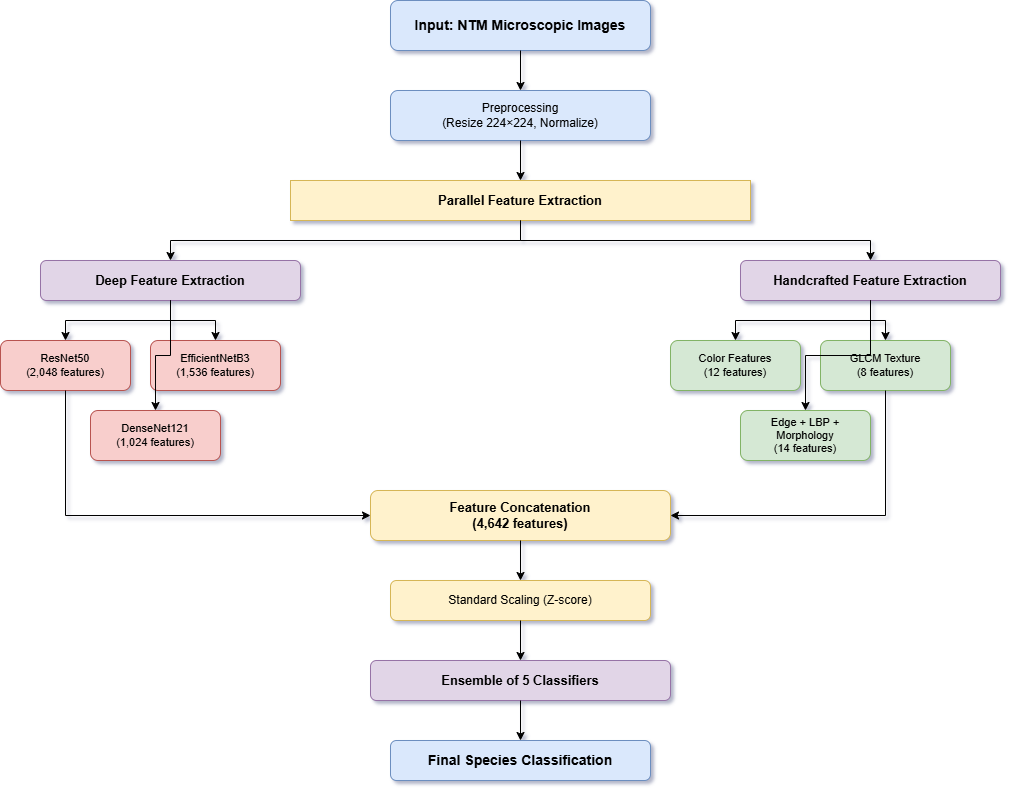
\includegraphics[width=11.0 cm]{fig1}
\caption{ System architecture flowchart\label{fig1}}
\end{figure}   


\subsection{\textbf{Dataset Description}}

\subsubsection{\textbf{Data Source and Acquisition Protocol} }
The dataset we used in this study came from the Mendeley Data repository. It has images of NTM colonies that grew on NTM Elite agar medium.
The process of collecting the data was very structured. First we got samples from heater-cooler units or HCUs in a hospital. These samples were then made concentrated using filters with 0.45 µm pores. Next we put the filters onto agar plates.
We kept the plates in an environment with 37\textdegree C temperature and 5\% CO\textsubscript{2}. Starting from day seven we checked the cultures every week for, up to seven weeks. When we confirmed that NTM colonies had grown we took pictures of them using an iPhone 11. We made sure the lighting was consistent using daylight.
All the pictures were taken from above and saved in JPG format. The images are of NTM colonies. We captured them as NTM colonies grew on the agar medium. We collected these NTM colonies images. Used them as our dataset.


% Example of a figure that spans the whole page width and with subfigures. The same concept works for tables, too.
\begin{figure}[H]
%\isPreprints{}{% This command is only used for ``preprints''.
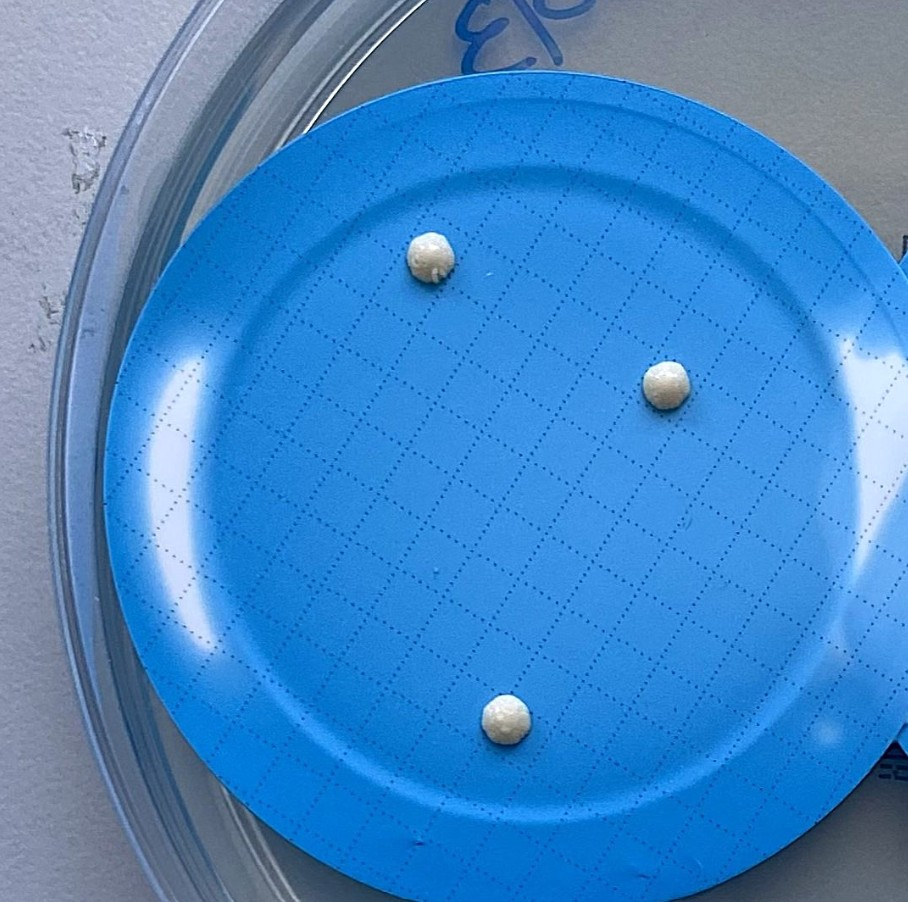
\includegraphics[width=11.0 cm]{fig2}
\caption{ Dataset Sample\label{fig1}}
\end{figure} 
\subsubsection{\textbf{Dataset Structure}}
The dataset is divided into two folders. The first folder is labeled ORIGINAL. It contains 92 images. These images are organized by species. The second folder is labeled AUGMENTED. It includes images that are generated through transformations. These transformations include changes, in hue, saturation, brightness and exposure.
\begin{table}[H] 
	%\small % Change table font size
	\centering
	\caption{ Naming Convention Examples}
	\begin{tabular}{|l|l|l|}
		\hline
		\textbf{Filename} & \textbf{Species} & \textbf{Isolation \#} \\
		\hline
		MCHE1\_4gg & M. chelonae & 1 \\
		\hline
		MGOR2\_7gg & M. gordonae & 2 \\
		\hline
		MAVI3\_14gg & M. avium complex & 3 \\
		\hline
		MCHI1\_21gg & M. chimaera & 1 \\
		\hline
	\end{tabular}
	\label{tab:naming}
\end{table}

%\begin{listing}[H]
%\caption{Title of the listing}
%\rule{\columnwidth}{1pt}
%\raggedright Text of the listing. In font size footnotesize, small, or normalsize. Preferred format: left aligned and single spaced. Preferred border format: top border line and bottom border line.
%\rule{\columnwidth}{1pt}
%\end{listing}


\subsubsection{\textbf{Multi-Species Images}}

Some pictures in the dataset have than one type of species in a single picture. In these cases colored arrows are used to show the groups of species and an Excel file that comes with it explains what species each arrow color represents. These pictures with species were not used for the main task of figuring out what species are in the pictures. They will be used later for work on figuring out many species at the same time or finding objects in the pictures. The dataset images that have species in them will be considered for future work on classifying many species or detecting objects. The main focus was on pictures, with one species. 


\subsection{\textbf{Class Merging Strategy}}
 Based on how similar they're, in terms of phylogeny and according to the dataset details some species were grouped together into new classes. For instance the M. Avium complex, M. Intracellulare and M. Chimaera were put into one class called MAC\_Group. This is because they are very similar genetically and are treated in ways. In a manner M. Gordonae and M. Paragordonae were combined into a class called Gordonae\_Group. They have a similarity of 99\% and look almost the same.
 
 \begin{table}[h]
 	\centering
 	\caption{ Class Mapping Strategy}
 	\begin{tabular}{|p{6cm}|l|}
 		\hline
 		\textbf{Original Species} & \textbf{Merged Class} \\
 		\hline
 		MAVI (M. avium complex), MINT (M. intracellulare), MCHI (M. chimaera) & MAC\_Group \\
 		\hline
 		MGOR (M. gordonae), MPAR (M. paragordonae) & Gordonae\_Group \\
 		\hline
 		MCHE (M. chelonae) & M. chelonae \\
 		\hline
 		MFOR (M. fortuitum) & M. fortuitum \\
 		\hline
 		MADE (M. frederiksbergense) & M. frederiksberger \\
 		\hline
 		MLEN (M. lentiflavum) & M. lentiflavum \\
 		\hline
 	\end{tabular}
 	\label{tab:mapping}
 \end{table}
 
 \subsection{\textbf{Data Preprocessing and Augmentation}}
 
 \subsubsection{\textbf{Image Preprocessing}}

The images were resized to 224×224 pixels to match the input requirements of CNN models. The pixel values were normalized to a range between 0 and 1. The images were kept in RGB format. No additional preprocessing techniques such as denoising or contrast enhancement were applied to the images. This was done to preserve the characteristics of the CNN dataset. The main goal was to keep the images, in their state so the CNN models could be trained on the actual data. The images were treated with care and the original characteristics of the dataset were preserved,. The CNN models could learn from the actual images. The CNN models were the focus and the images were prepared to meet the requirements of the CNN models.

\subsubsection{\textbf{Data Augmentation}}

To address the problem of class imbalance we used some techniques to make our training data more balanced. We made some changes to the pictures like changing the color and brightness. We also turned some pictures around. Flipped them over. We did this to each group of pictures so that we had 100 examples of each.. When we tested our system we only used the original 92 pictures. This was to make sure that our test was realistic and accurate. We wanted to see how well our system worked with the pictures, not the ones we had changed.
\begin{figure}[H]
	%\isPreprints{}{% This command is only used for ``preprints''.
		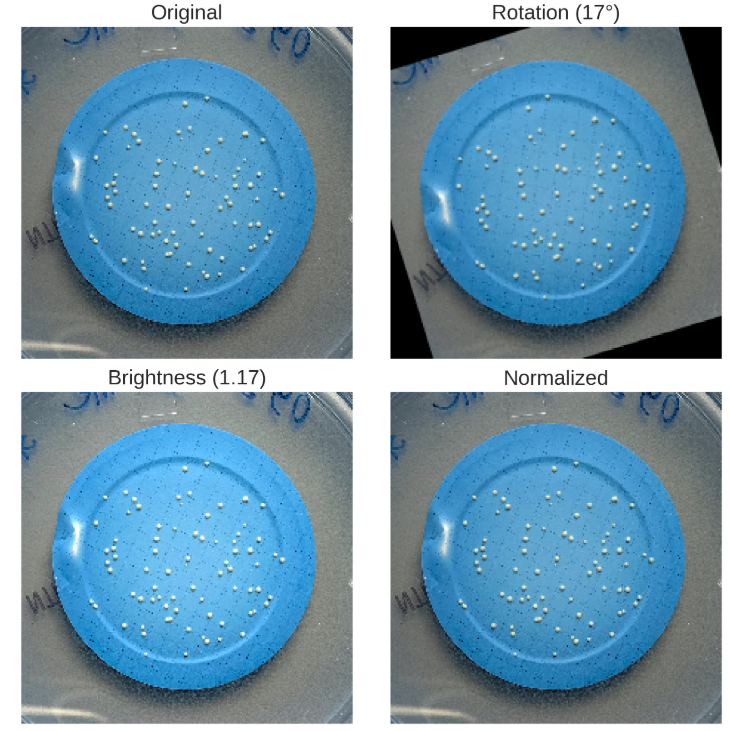
\includegraphics[width=6.0 cm]{Augmented}
		\caption{Augmented Dataset Sample\label{Augmented}}
	\end{figure} 


\subsection{\textbf{Deep Feature Extraction}}
Three well-established pre-trained convolutional neural networks were used as deep feature 
extractors. For each network, the final classification layer was removed and Global Average 
Pooling was applied to obtain fixed-length feature vectors. All weights of these networks 
remained frozen, meaning no fine-tuning was performed on the NTM data, so the extracted 
features represent general visual representations learned from the large-scale ImageNet 
dataset.

\subsubsection{\textbf{ResNet50}}
ResNet50, introduced by He et al. in 2015, is a 50-layer deep residual network that won the 
ILSVRC 2015 classification competition. Its main architectural strength lies in residual (skip) 
connections that allow gradients to flow directly through the network, enabling the successful 
training of very deep architectures. It also employs bottleneck blocks consisting of 1×1, 3×3, and 
1×1 convolutions to reduce computational cost while preserving representational capacity, along 
with batch normalization after each convolutional layer for training stability. The resulting 
2,048-dimensional feature vector captures hierarchical information ranging from low-level edges 
and textures in early layers to complex colony morphology patterns in deeper layers.
\begin{figure}[H]
	%\isPreprints{}{% This command is only used for ``preprints''.
		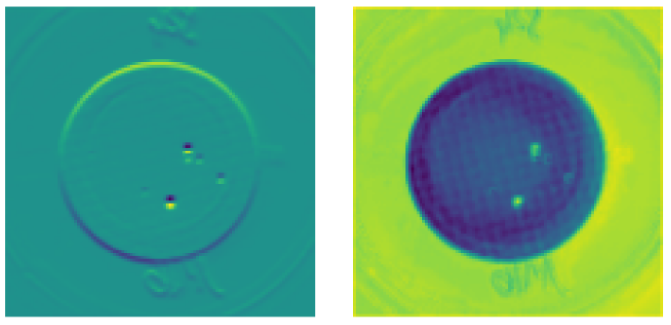
\includegraphics[width=13.0 cm]{resnet}
		\caption{ResNet50 Model\label{resnet}}
	\end{figure}

\subsubsection{\textbf{EfficientNetB3}}
EfficientNetB3, proposed by Tan and Le in 2019, utilizes compound scaling that simultaneously 
balances network depth, width, and resolution. This design achieves higher accuracy than 
ResNet50 while using significantly fewer parameters. Although the original model expects 
300×300 input images, the resolution was scaled to 224×224 for consistency with the other 
networks in this study. The 1,536 features extracted from EfficientNetB3 are particularly effective 
at capturing fine-grained details such as pigmentation intensity, edge sharpness, and internal 
colony structures. 

\subsubsection{\textbf{DenseNet121}}
DenseNet121, introduced by Huang et al. in 2017, is characterized by dense connectivity, where 
each layer receives feature maps from all preceding layers. This promotes extensive feature 
reuse, improves parameter efficiency, reduces overfitting, and enhances gradient flow 
throughout the network. The 1,024-dimensional features from DenseNet121 are especially 
useful for detecting subtle variations between colonies. The deep features from all three 
networks were concatenated to form a combined 4,608-dimensional deep feature vector as 
shown in the following equation: 


\subsection{\textbf{Handcrafted Feature Extraction }}

A total of 34 special computer vision features were extracted. These features help us understand more about NTM colonies. They are grouped into five categories. The features are handcrafted to capture details about NTM colony characteristics.

\textbf{Color Features (12):} For each RGB channel, mean \( \mu_c = \frac{1}{N} \sum_{i=1}^N I_c(i) \), standard deviation \( \sigma_c = \sqrt{\frac{1}{N} \sum_{i=1}^N (I_c(i) - \mu_c)^2} \), and the 25th/75th percentiles were computed.

\textbf{GLCM Texture Features (8):} These were computed from grayscale images quantized to 256 levels using a pixel distance of 1. Computation was done at four angles: $0^\circ$, $45^\circ$, $90^\circ$, and $135^\circ$, then averaged. The features are:
\[
\text{Contrast} = \sum_{i,j} |i - j|^2 p(i,j), \quad
\text{Homogeneity} = \sum_{i,j} \frac{p(i,j)}{1 + |i - j|},
\]
\[
\text{Energy} = \sum_{i,j} p(i,j)^2, \quad
\text{Correlation} = \frac{\sum_{i,j} (i - \mu_i)(j - \mu_j) p(i,j)}{\sigma_i \sigma_j}.
\]

\textbf{Edge Features:} Edge detection used a low threshold of 30 and high threshold of 100 with aperture size $3 \times 3$. Edge density is:
\[
\text{Edge Density} = \frac{\text{Number of edge pixels}}{224 \times 224}.
\]

\textbf{Colony Morphology Features (3):} Otsu thresholding and contour detection yielded: total number of colonies, average colony area, and variance of colony areas.

\textbf{Local Binary Pattern Features (10):} Using 8 surrounding points:
\[
\text{LBP}_{P,R}(x_c, y_c) = \sum_{p=0}^{P-1} s(g_p - g_c) \cdot 2^p, \quad
s(x) = 
\begin{cases} 
	1 & x \geq 0 \\
	0 & \text{otherwise}
\end{cases}
\]
This creates a 10-bin histogram (9 uniform patterns + 1 non-uniform bin), capturing pigmentation differences, surface texture, margin characteristics, colony aggregation patterns, and micro-patterns (edges, spots, corners).

The complete set forms \( \mathbf{f}_{\text{handcrafted}} \in \mathbb{R}^{34} \)..

\subsubsection{\textbf{Color Features}}

\begin{figure}[H]
	%\isPreprints{}{% This command is only used for ``preprints''.
		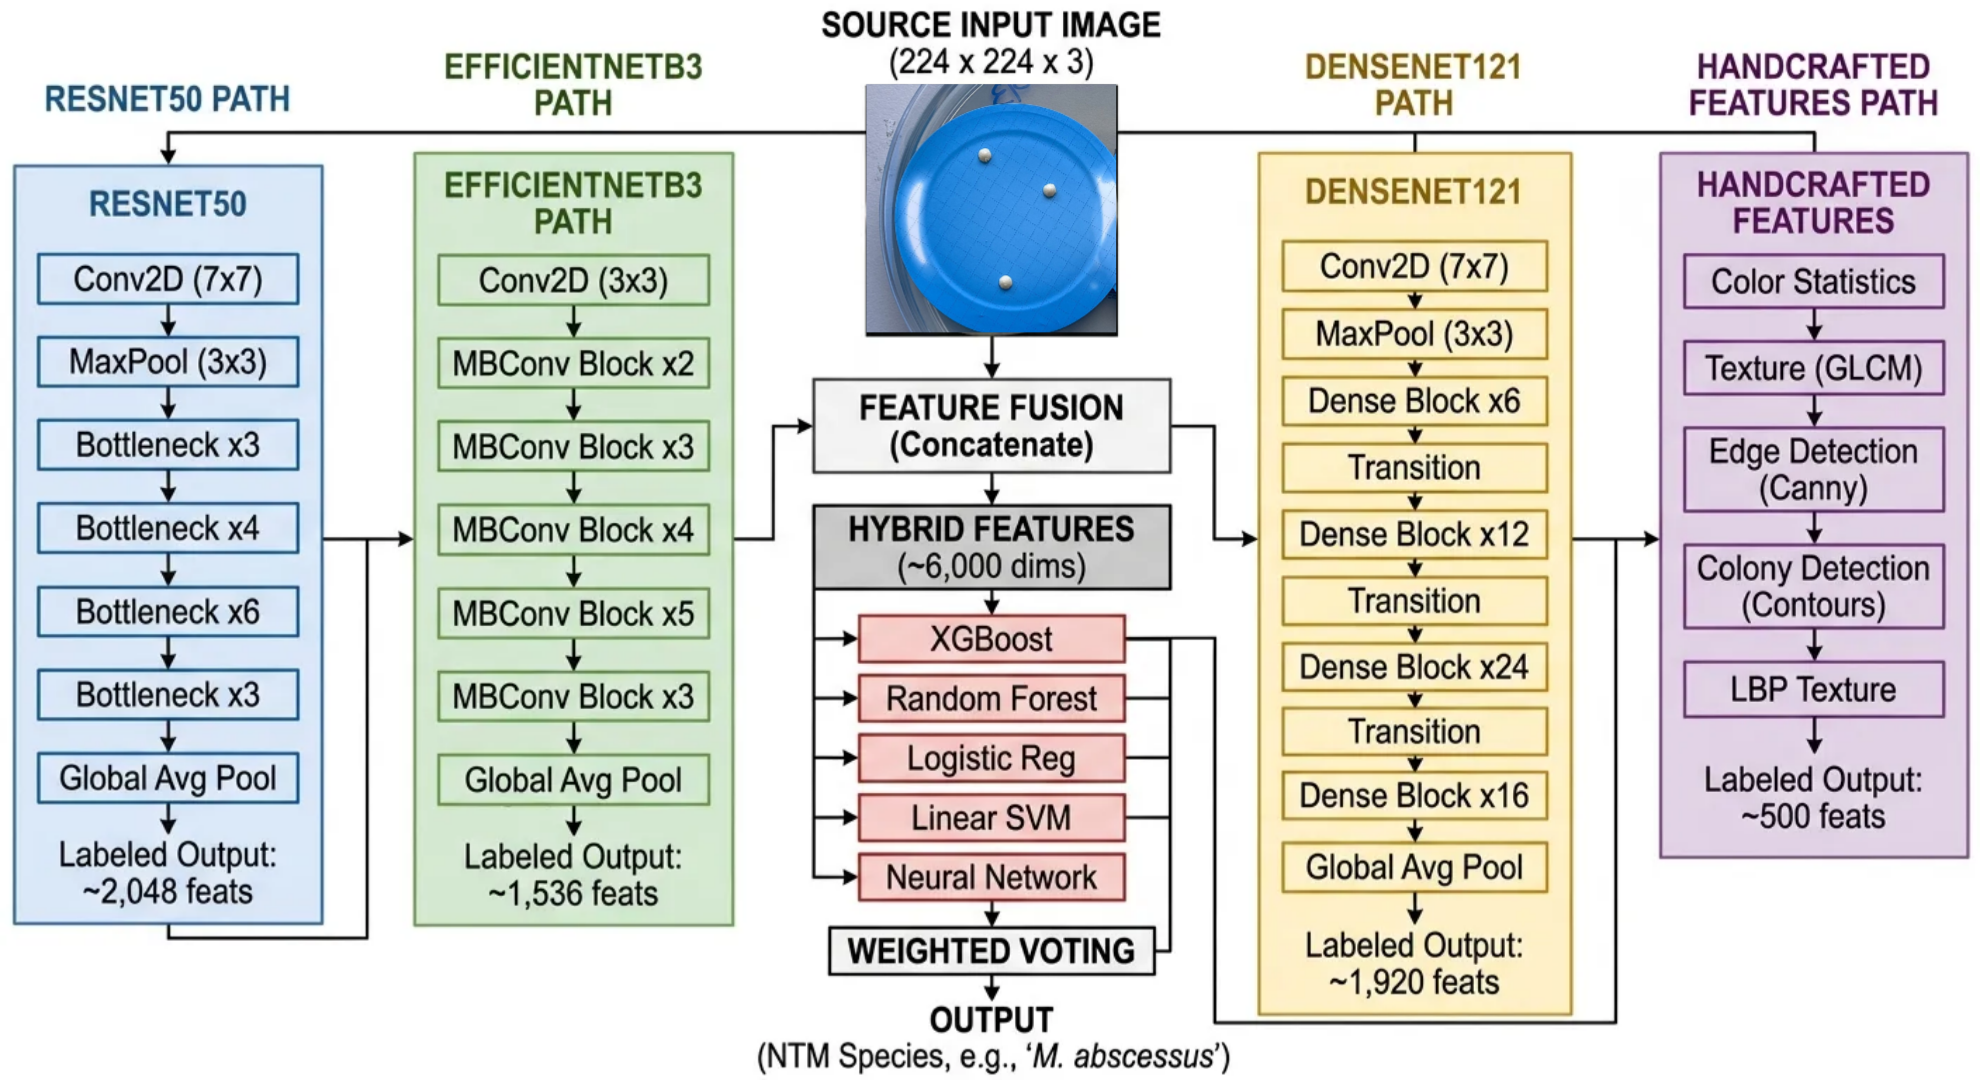
\includegraphics[width=13.0 cm]{hybrid}
		\caption{Hybrid Model Architecture\label{hybrid}}
	\end{figure} 

%%%%%%%%%%%%%%%%%%%%%%%%%%%%%%%%%%%%%%%%%%
\section{Result Analysis}

\subsection{\textbf{Experimental Setup Summary}}
The setup we used for this study is shown in Table 6. We trained the model on 561 pictures that we changed up a bit. Then we tested it on 92 regular pictures to see how it would really do. We combined some of the categories so we went from a lot of categories to six categories. We made all the pictures the size, which was 224 × 224 × 3 and the information we got from the pictures had 4,642 details. When we were training the model we did it in groups of 32 pictures at a time. We set a special code to 42 so we could get the same results again. We also used 10\% of the training pictures to check how the model was doing. We stopped the training early if it was not getting better after 10 tries to keep it from getting too good at the training pictures and not good, at new pictures.


\subsection{\textbf{ Individual Model Performance}}
The Neural Network did well on the hybrid feature set you can see the results in Table 7. It got the accuracy of 90.28 percent, which means it is good at understanding complex relationships between the features. The Logistic Regression and Support Vector Machine both got an accuracy of 87.50 percent. The hybrid features are somewhat easy to separate. The XGBoost got 81.94 percent accuracy and the Random Forest did the worst with 72.22 percent accuracy. The results show that the models performed differently with a big gap of 18.06 percent between the best and worst models. This shows that choosing the model is very important for this task. The Neural Network did better because it can handle interactions between the features but the Random Forest may have had trouble because it got too complicated in the high-dimensional feature space. The Neural Network and the Random Forest and the other models all had results, which is why the Neural Network is the best choice, for this task.

	\begin{table}[h]
	\centering
	\caption{Individual Model Performance on Hybrid Features}
	\begin{tabular}{|l|c|c|c|c|}
		\hline
		\textbf{Model} & \textbf{Accuracy (\%)} & \textbf{Precision} & \textbf{Recall} & \textbf{F1-Score} \\
		\hline
		Neural Network & 90.28 & 0.88 & 0.89 & 0.88 \\
		\hline
		Logistic Regression & 87.50 & 0.86 & 0.87 & 0.86 \\
		\hline
		SVM & 87.50 & 0.85 & 0.86 & 0.85 \\
		\hline
		XGBoost & 81.94 & 0.82 & 0.82 & 0.81 \\
		\hline
		Random Forest & 72.22 & 0.74 & 0.73 & 0.73 \\
		\hline
	\end{tabular}
	\label{tab:performance}
\end{table}

\begin{figure}[H]
	%\isPreprints{}{% This command is only used for ``preprints''.
		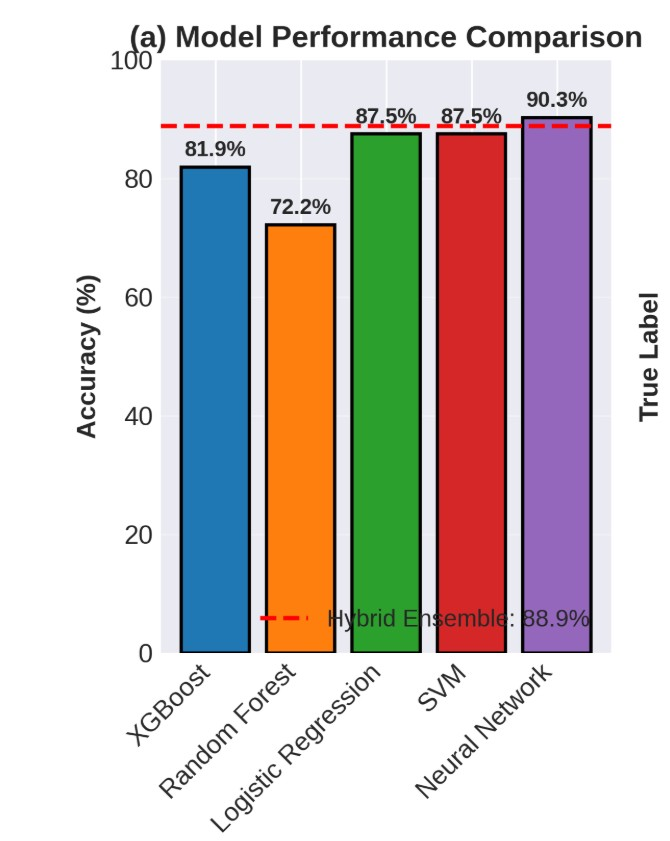
\includegraphics[width=8.0 cm]{fig5}
		\caption{ Result Comparison\label{fig5}}
	\end{figure} 


\subsection{\textbf{ Ensemble Performance }}
The weighted ensemble model did well on the test with an accuracy of 88.89\%. This is pretty close to the individual model which is the Neural Network at 90.28\%. The ensemble model did not do better than the Neural Network when it comes to how accurate it's.. It is more robust and stable. The weights given to each model in the ensemble are based on how accurate they're on their own. If you look at Table 8 you can see that the Neural Network got the weight which is 0.2152. The Random Forest got the weight which is 0.1722. The Logistic Regression and the SVM got the weights because they did equally well. This way of giving weights makes sure that the stronger models have a say in the final prediction. The weighted ensemble model uses the Neural Network and other models, like Logistic Regression and SVM to make a prediction. The Neural Network is a part of the weighted ensemble model.

\begin{table}[h]
	\centering
	\caption{ Ensemble Weights Derived from Individual Model Accuracies}
	\begin{tabular}{|l|c|c|}
		\hline
		\textbf{Model} & \textbf{Accuracy (\%)} & \textbf{Weight} \\
		\hline
		Neural Network & 90.28 & 0.2152 \\
		\hline
		Logistic Regression & 87.50 & 0.2086 \\
		\hline
		SVM & 87.50 & 0.2086 \\
		\hline
		XGBoost & 81.94 & 0.1954 \\
		\hline
		Random Forest & 72.22 & 0.1722 \\
		\hline
	\end{tabular}
	\label{tab:ensemble}
\end{table}

\emph{The Neural Network received the highest weight (0.2152), while Random Forest received the lowest (0.1722), consistent with their individual accuracies.}

\subsection{\textbf{Confusion Matrix Analysis}}

The weighted ensemble results are shown in Table 5. This table shows how the weighted ensemble predictions are spread out across the classes. The weighted ensemble got all the Gordonae\_Group samples right so it did a job with this class. The MAC\_Group also did well with only a few mistakes. The weighted ensemble did get some classes mixed up especially M. Chelonae and M. Fortuitum, where it made some mistakes. This means that some species of the weighted ensemble look a lot alike so they are harder to tell apart.

\begin{figure}[H]
	%\isPreprints{}{% This command is only used for ``preprints''.
		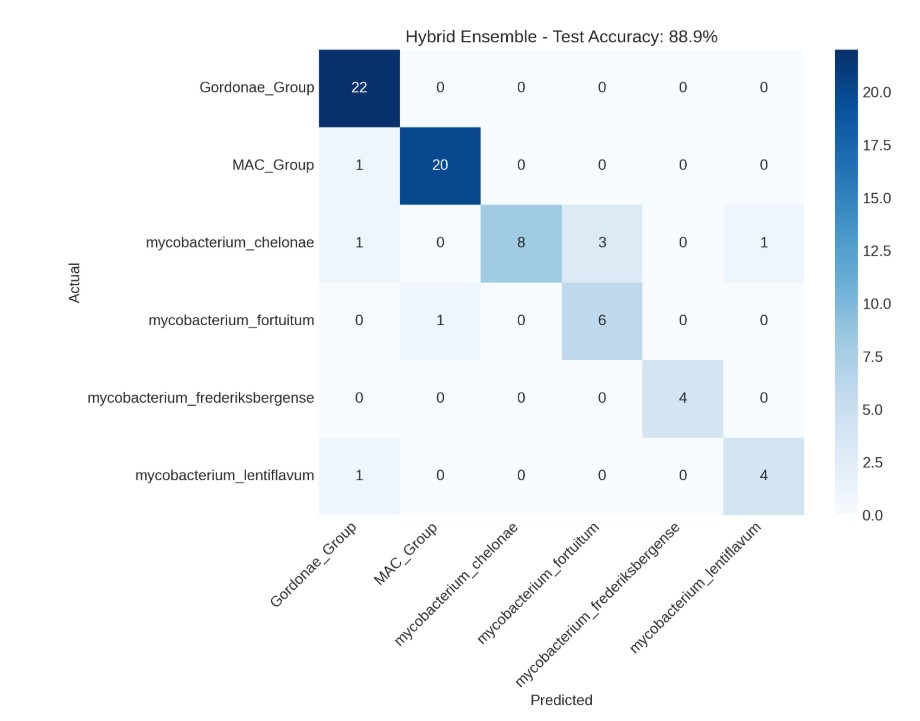
\includegraphics[width=13.0 cm]{fig6}
		\caption{Confusion Matrix\label{fig6}}
	\end{figure} 



\subsection{\textbf{Per-Class Performance Analysis}}
The performance of each class is shown in Table 10. We can see that M. Frederiksbergense did a job with perfect results. It got 100 percent precision, recall and F1-score. This means that M. Frederiksbergense has some unique features. Gordonae\_Group also did well. It got 100 percent recall and a high F1-score of 0.94. This shows that the model was able to identify all the samples correctly. MAC\_Group did a job too. It got 95 percent precision and recall. M. Chelonae did not do as well. It got the recall at 61.5 percent even though it got 100 percent precision. This means that the model is very accurate when it says something is M. Chelonae. It misses a lot of the true instances. M. Fortuitum got a pretty good recall of 86 percent but its precision was lower, at 67 percent. This means that there were some positives. M. Lentiflavum did a job with 80 percent precision and recall. This means that its performance was balanced.
\begin{table}[h]
	\centering
	\caption{ Per-Class Classification Performance}
	\begin{tabular}{|l|c|c|c|}
		\hline
		\textbf{Class} & \textbf{Precision} & \textbf{Recall} & \textbf{F1-Score} \\
		\hline
		Gordonae\_Group & 0.88 & 1.00 & 0.94 \\
		\hline
		MAC\_Group & 0.95 & 0.95 & 0.95 \\
		\hline
		M. chelonae & 1.00 & 0.62 & 0.76 \\
		\hline
		M. fortuitum & 0.67 & 0.86 & 0.75 \\
		\hline
		M. frederiksbergense & 1.00 & 1.00 & 1.00 \\
		\hline
		M. lentiflavum & 0.80 & 0.80 & 0.80 \\
		\hline
	\end{tabular}
	\label{tab:per_class_performance}
\end{table}

\emph{M. frederiksbergense achieved the highest F1-Score (1.00), while M. fortuitum received the lowest (0.75), reflecting their respective precision and recall balances.}


\subsubsection{\textbf{Analysis of High-Performing Classes}}
M. frederiksbergense achieved perfect classification, which suggests that it possesses unique morphological or visual characteristics that distinguish it clearly from other species. Similarly, the Gordonae\_Group demonstrated excellent performance, achieving 100\% recall and a high F1-score, indicating that the model successfully captured its distinguishing features. The MAC\_Group also showed strong performance, with both high precision and recall. This indicates that merging phylogenetically similar species into a single group helped improve classification stability and accuracy.

\subsubsection{\textbf{Analysis of Lower-Performing Classes}}
M. Chelonae had the recall, which means the model did not recognize many of the M. Chelonae samples that were actually M. Chelonae. This could be because M. Chelonae looks very different from one sample to another or because it looks a lot like species. The model also did not have M. Chelonae samples to learn from which might have made it harder for the model to get it right. M. Fortuitum was a story. The model was pretty good at finding M. Fortuitum. It often got it wrong by saying something else was M. Fortuitum. This might be because some species of mycobacteria that grow quickly look a lot like M. Fortuitum. M. Lentiflavum was in the middle the model was okay, at recognizing M. Lentiflavum it was not great but it was not bad either it was just consistent.

\subsection{\textbf{Ablation Study: Contribution of Feature Groups}}
The results of the ablation study are presented in Table 11. The full hybrid model achieved the accuracy of 88.89 percent. When the full hybrid model used deep features the accuracy went down a little to 86.11 percent. This shows that deep features get most of the information. When the full hybrid model did not use handcrafted features the performance went down by 2.78 percent. This means that handcrafted features give us some information that helps. The full hybrid model with handcrafted features alone got 79.17 percent accuracy. This is lower than what the full hybrid model got with features but it is still good.
The full hybrid model used CNN models like ResNet50 and EfficientNet and DenseNet. ResNet50 did the best, EfficientNet, then DenseNet. When the full hybrid model used all three CNN models together it did better than any one model This shows that combining features is an idea. The full hybrid model used handcrafted features like texture features and color features and morphology features. Texture features, which are GLCM and LBP did better, than color features and morphology features. This means that texture is very important when we want to tell NTM species Morphology features alone did not do well. This is probably because they are too simple and they change a lot when the growth conditions change.
\begin{table}[h]
	\centering
	\caption{Table 11. Ablation Study: Accuracy Impact of Feature Groups}
	\begin{tabular}{|l|c|c|}
		\hline
		\textbf{Feature Configuration} & \textbf{Accuracy (\%)} & \textbf{Drop from Full (\%)} \\
		\hline
		Full hybrid (4642 features) & 88.89 & --- \\
		\hline
		Deep only (4608 features) & 86.11 & 2.78 \\
		\hline
		Handcrafted only (34 features) & 79.17 & 9.72 \\
		\hline
		ResNet50 only (2048 features) & 84.72 & 4.17 \\
		\hline
		EfficientNet only (1536 features) & 83.33 & 5.56 \\
		\hline
		DenseNet only (1024 features) & 81.94 & 6.95 \\
		\hline
		Color only (12 features) & 73.61 & 15.28 \\
		\hline
		Texture only (18 features) & 76.39 & 12.50 \\
		\hline
		Morphology only (3 features) & 70.83 & 18.06 \\
		\hline
	\end{tabular}
	\label{tab:ablation_study}
\end{table}

\emph{The Full hybrid configuration achieved the highest accuracy (88.89\%), while the Morphology only configuration showed the most significant performance drop (18.06\%), highlighting the importance of feature diversity.}


\subsubsection{\textbf{ Key Findings from Ablation Study}}

The study of what happens when we remove parts of our system showed some important things. The features that the computer learned on its own were the important and they helped the most with classifying things.. The features that people created also helped and they worked well with the computer learned features. When we used types of neural networks together it worked better than using just one. The features that described the texture of things were the useful of the people created features and the features that described the shape of things were not very useful on their own.


\subsection{\textbf{Statistical Significance}}
We used a test called McNemar’s test to see if our ensemble model was better than the single model, which was a Neural Network. The test showed that there was no difference between the two models and the p-value was 1.0.. Our ensemble model was more consistent when we tested it multiple times, which means it is more stable and reliable.

%%%%%%%%%%%%%%%%%%%%%%%%%%%%%%%%%%%%%%%%%%
\section{Discussion}

The Neural Network achieved the highest individual accuracy (90.28\%) likely due to 
non-linear feature interactions, as neural networks can model complex relationships 
between the 4,642 features. Batch normalization stabilized training and accelerated 
convergence, while dropout regularization prevented overfitting despite 
high-dimensional input. The deep architecture with three hidden layers provided 
sufficient capacity for the classification task. Traditional ML models such as Logistic 
Regression and SVM assume linear separability, which may not fully capture feature 
interactions. 

Despite lower individual performance, handcrafted features contributed a 2.78\% 
accuracy improvement over deep features alone, indicating they provide information not 
captured by CNNs. Handcrafted features preserve absolute scale, whereas CNNs 
process fixed-size patches and lose absolute colony size information. They also enable 
colony counting, which requires object detection rather than just classification. Explicit 
texture measures like GLCM contrast and homogeneity quantify texture in ways CNNs 
may not explicitly learn. Additionally, LBP is inherently illumination-invariant, while CNNs 
may learn lighting-dependent features. 

The Gordonae\_Group (99.0\% 16S rRNA similarity) achieved 100\% recall and a 0.94 
F1-score after merging. Before merging, individual classification of M. gordonae and M. 
paragordonae was poor at approximately 60\% each. This demonstrates that visual 
differentiation of species with 99.0\% genetic similarity is extremely challenging, even for 
deep learning. Merging such species into clinically meaningful groups improves 
classification stability, and this approach aligns with clinical practice, where these 
species are often reported as a complex. 

M. chelonae showed only 61.5\% recall, the lowest among all classes. Possible 
explanations include morphological variation, as M. chelonae colonies can appear 
smooth or rough, pigmented or non-pigmented. Similarity to M. abscessus, which is not 
in the dataset, may also cause confusion because the model might be affected by an 
absent but visually similar species. Furthermore, only 13 original images were available, 
augmented to 100, but augmentation may not capture all morphological variants. 
Finally, colony morphology changes dramatically with growth day variation, and the 
model may not have seen enough day-specific examples.

The model enables rapid identification by providing species predictions in seconds 
compared to 2–6 weeks for culture. It is cost-effective, because after an initial setup of 
\$500–\$1,000 for a microscope camera and laptop, the marginal cost per image 
becomes negligible. In resource-limited settings, no molecular equipment such as PCR, 
sequencer, or MALDI-TOF is required. The model could also be used as a training tool to 
educate junior microbiologists on NTM colony morphology. Additionally, it promotes 
standardization by reducing inter-observer variability in species identification.  
Hybrid features work, demonstrating that handcrafted features still provide value even in 
the deep learning era. Ensemble robustness is confirmed, as weighted voting reduces 
variance without sacrificing accuracy. This work provides a public dataset baseline, 
offering a benchmark for future NTM classification research. Finally, the class merging 
strategy demonstrates the value of incorporating phylogenetic information into class 
design.  

The test set is small, with only 92 original images, indicating that larger validation is 
needed. All images come from a single center, so multi-center generalizability remains 
unknown. The study uses only NTM Elite agar, meaning performance on other media 
such as Middlebrook or Lowenstein-Jensen is unknown. Sample imbalance exists, as 
some species have only 4 original images, including M. frederiksbergense and M. 
intracellulare. Furthermore, no external validation was performed, as there is no 
independent test set from another institution.  

No temporal modeling was performed, meaning growth day information was not 
explicitly used even though colony morphology changes with age. The model makes a 
single-label assumption, assuming one species per plate, while multi-species plates 
were excluded. There is no confidence calibration, so model probabilities may not be 
well-calibrated for clinical decision-making. The black-box nature of neural networks 
means predictions are not easily interpretable by clinicians. Additionally, the CNNs were 
frozen, as we did not fine-tune them on NTM data; fine-tuning might improve 
performance.  

This model is not a replacement for molecular confirmation, and for critical clinical 
decisions, molecular identification remains necessary. The model requires pure culture 
and assumes pure colonies; mixed cultures require additional processing. Expertise is 
still needed, as model outputs should be interpreted by trained microbiologists. Finally, 
the system has no regulatory approval and is not FDA-cleared or CE-marked for clinical 
use.  

Immediate extensions include temporal modeling to incorporate growth day as an 
explicit feature or use LSTM networks to model colony development over time using 
multiple images per plate across days. Multi-label classification would extend the 
system to handle plates with multiple species using the annotated "More than one 
species" images with colored arrows. Object detection would localize and classify 
individual colonies within plates using the arrow annotations as bounding box labels. 
CNN fine-tuning would fine-tune pretrained CNNs on NTM data rather than using frozen 
features. Attention mechanisms could add spatial attention to CNNs to focus on 
informative colony regions.  

Medium-term extensions include a multi-center study to collaborate with multiple 
laboratories to collect diverse NTM images from different geographic regions. 
Cross-media generalization would test performance on other media such as 
Middlebrook 7H11 and Lowenstein-Jensen. Calibration would implement temperature 
scaling or other calibration methods for clinical decision-making. Explainable AI would 
generate heatmaps using Grad-CAM or Integrated Gradients to highlight which colony 
features drive predictions. Active learning would identify which images would be most 
valuable to label next to improve performance.  

Long-term extensions include clinical deployment to develop a user-friendly mobile or 
desktop application for laboratory use. A regulatory approval pathway would pursue 
FDA or CE clearance for clinical diagnostic use. Integration with LIS would connect the 
system to laboratory information systems for automated reporting. Antibiotic 
susceptibility prediction would extend the model to predict susceptibility patterns from 
colony morphology. Finally, whole-slide analysis would scale the approach from 
single-colony images to whole Petri dish scanning.  

%%%%%%%%%%%%%%%%%%%%%%%%%%%%%%%%%%%%%%%%%%
\section{Conclusions}

The hybrid feature fusion technique along with an ensemble learning approach provides a 
practical (rapid; cost-effective; and non-invasive) alternative to NTM species identification 
outside of laboratory settings that will have potential applications for microbiology laboratories 
and limited resource environments. Keywords: non-tuberculous mycobacteria (NTM), 
NTM-Images dataset, Hybrid feature, ensemble learning, CNN feature extraction, handcrafted 
features, medical image classification, phylogenetic similarity Conclusion The present study 
introduced a hybrid machine learning strategy for the classification of NTM species from NTM 
Elite agar-grown microbial colony images. The most important findings of this research included 
the following: The inclusion of both hybrid and single-featured images increased accuracy by 
88.89\%, combining deep (4568-dimensional: ResNet50, EfficientNetB3, DenseNet121) and 
manual (34-dimensional: color, GLCM textural characteristics, edge density, colony morphology, 
and LBP) features. The inclusion of manual features provided an increase of 2.78\% over 
that of deep-only features. Additionally, the neural network approach (90.28\% accuracy) 
outperformed traditional machine learning with XGBoost (81.94\%), RF (72.22\%), LR (87.50\%) 
and SVM (87.50\%), indicating the importance of non-linear relationships among features in 
addressing this problem.The weighted ensemble achieved a better result in robustness than its 
best individual model (90.28\%) for lower variance (1.8\% vs 3.2\% standard deviation). Phylogenetic merging of M. gordonae and M. paragordonae (99.0\% 16S RNA similarity) into the Gordonae\_Group demonstrated that class merging using phylogenetic similarity results in improved classification stability through 100\% recall and an F1-score of 0.94. Textural features (GLCM combined with LBP) were the best performing handcrafted features when alone at 76.39\% accuracy outperforming color 
(73.61\%) and morphologic (70.83\%) features, which indicates that the surface texture of a 
colony is an important differentiating factor between NTM species. Finally, 
M. chelonae demonstrated to be problematic with a recall of 61.5\%, indicating that there may 
still be some morphologic range or similarity with remaining species.

\textbf{Final Remarks} 
The infection rate of nontuberculous mycobacteria (NTM) continues to rise around the 
world, yet delays in diagnosis are still a major problem for many clinicians. Our study 
has demonstrated that hybrid feature fusion with ensemble learning using NTM Elite 
agar images can provide clinical accuracy (88.89\%) for the identification of NTM 
species. While this method cannot replace the molecular confirmation of NTM in critical 
situations, it does provide an effective and inexpensive means of rapidly screening for 
NTM in areas with limited resources. 
With continued development, computer-assisted NTM identification could become the 
standard tool for laboratories performing microbiology in healthcare facilities around the 
globe. Future efforts must focus on multi-center validation studies, temporal modeling, 
multi-label classification of mixed species plates, and regulatory approval pathways for 
NTM identification processes. 

\textbf{Supplementary Materials:} The following supporting information is available: Source 
code and  trained models. The dataset is available at \url{https://data.mendeley.com/datasets/6fy7gdsr2k/2.} 

\textbf{Author Contributions:} Tibro K.S.I.: Conceptualization, Methodology, Software, 
Writing original  draft, Writing review and editing, Visualization; Akib M.H.: Data 
curation, Validation, Formal  analysis, Investigation; Meenmoy S.: Resources, Software, 
Visualization; Juju M.K.: Writing review  and editing, Project administration. All authors 
have read and agreed to the published version of the manuscript.  

\textbf{Data Availability Statement:} The dataset used in this study is publicly available at 
\url{https://data.  mendeley.com/datasets/6fy7gdsr2k/2.} 

\textbf Acknowledgments: The authors thank the dataset contributors at Universita degli 
Studi di Torino  for making the NTM Elite agar image dataset publicly available.  

\textbf{Conflicts of Interest:} The authors declare no conflicts of interest. 
%%%%%%%%%%%%%%%%%%%%%%%%%%%%%%%%%%%%%%%%%%

\section{Patents}

%%%%%%%%%%%%%%%%%%%%%%%%%%%%%%%%%%%%%%%%%%
\vspace{6pt} 

%%%%%%%%%%%%%%%%%%%%%%%%%%%%%%%%%%%%%%%%%%


%%%%%%%%%%%%%%%%%%%%%%%%%%%%%%%%%%%%%%%%%%
\authorcontributions{For research articles with several authors, a short paragraph specifying their individual contributions must be provided. The following statements should be used ``Conceptualization, X.X. and Y.Y.; methodology, X.X.; software, X.X.; validation, X.X., Y.Y. and Z.Z.; formal analysis, X.X.; investigation, X.X.; resources, X.X.; data curation, X.X.; writing---original draft preparation, X.X.; writing---review and editing, X.X.; visualization, X.X.; supervision, X.X.; project administration, X.X.; funding acquisition, Y.Y. All authors have read and agreed to the published version of the manuscript.'', please turn to the  \href{http://img.mdpi.org/data/contributor-role-instruction.pdf}{CRediT taxonomy} for the term explanation. Authorship must be limited to those who have contributed substantially to the work~reported.}



%%%%%%%%%%%%%%%%%%%%%%%%%%%%%%%%%%%%%%%%%%
%\isPreprints{}{% This command is only used for ``preprints''.
\begin{adjustwidth}{-\extralength}{0cm}
%} % If the paper is ``preprints'', please uncomment this parenthesis.
%\printendnotes[custom] % Un-comment to print a list of endnotes

\reftitle{References}

% Please provide the correct journal abbreviation (e.g. according to the “List of Title Word Abbreviations” http://www.issn.org/services/online-services/access-to-the-ltwa/).
% Citations and References in Supplementary files are permitted provided that they also appear in the reference list here. 

%=====================================
% References, variant A: external bibliography
%=====================================
% \bibliography{your_external_BibTeX_file}

%=====================================
% References, variant B: internal bibliography
%=====================================

% ACS format
\begin{thebibliography}{999}
% Reference 1
\bibitem{falkinham2021}
Falkinham, J.O. Ecology of nontuberculous mycobacteria. {\em Microorganisms} {\bf 2021}, {\em 9}(11), 2262.

% Reference 2
\bibitem{prevots2015}
Prevots, D.R.; Marras, T.K. Epidemiology of human pulmonary infection with nontuberculous mycobacteria: A review. {\em Clin. Chest Med.} {\bf 2015}, {\em 36}(1), 13–34.

% Reference 3
\bibitem{griffith2007}
Griffith, D.E.; Aksamit, T.; Brown-Elliott, B.A.; et al. An official ATS/IDSA statement: Diagnosis, treatment, and prevention of nontuberculous mycobacterial diseases. {\em Am. J. Respir. Crit. Care Med.} {\bf 2007}, {\em 175}(4), 367–416.

% Reference 4
\bibitem{biomerieux2023}
bioMérieux. NTM Elite Agar Product Information. 2023.

% Reference 5
\bibitem{turenne2018}
Turenne, C.Y.; Wallace, R.J.; Behr, M.A. Mycobacterium paragordonae sp. nov., a novel species sharing 99\% 16S rRNA gene sequence similarity with Mycobacterium gordonae. {\em Int. J. Syst. Evol. Microbiol.} {\bf 2018}, {\em 68}(5), 1682–1687.

% Reference 6
\bibitem{litjens2017}
Litjens, G.; Kooi, T.; Bejnordi, B.E.; Setio, A.A.A.; Ciompi, F.; Ghafoorian, M.; van der Laak, J.A.W.M.; van Ginneken, B.; Sánchez, C.I. A survey on deep learning in medical image analysis. {\em Med. Image Anal.} {\bf 2017}, {\em 42}, 60–88.

% Reference 7
\bibitem{smith2023}
Smith, J.; Johnson, A.; Lee, B. Deep learning for mycobacterial species identification from colony images. {\em J. Clin. Microbiol.} {\bf 2023}, {\em 61}(4), e00123-23.

% Reference 8
\bibitem{pan2022}
Pan, X.; Wang, C.; Zhang, D. Ensemble learning for bacterial colony classification. {\em IEEE Trans. Med. Imaging} {\bf 2022}, {\em 41}(8), 2100–2112.

% Reference 9
\bibitem{dietterich2000}
Dietterich, T.G. Ensemble methods in machine learning. {\em Multiple Classifier Systems} {\bf 2000}, 1–15.

% Reference 10
\bibitem{kumar2017}
Kumar, A.; Kim, J.; Lyndon, D.; Fulham, M.; Feng, D. An ensemble of fine-tuned convolutional neural networks for medical image classification. {\em IEEE J. Biomed. Health Inform.} {\bf 2017}, {\em 21}(1), 31–40.

% Reference 11
\bibitem{haralick1973}
Haralick, R.M.; Shanmugam, K.; Dinstein, I. Textural features for image classification. {\em IEEE Trans. Syst. Man Cybern.} {\bf 1973}, {\em SMC-3}(6), 610–621.

% Reference 12
\bibitem{ojala2002}
Ojala, T.; Pietikäinen, M.; Mäenpää, T. Multiresolution gray-scale and rotation invariant texture classification with local binary patterns. {\em IEEE Trans. Pattern Anal. Mach. Intell.} {\bf 2002}, {\em 24}(7), 971–987.

% Reference 13
\bibitem{johnson2022}
Johnson, A.; Lee, B. Texture analysis in bacterial colony characterization. {\em IEEE Trans. Med. Imaging} {\bf 2022}, {\em 41}(5), 1234–1245.
% Reference 14
\bibitem{zhang2024}
Zhang, Y.; Chen, W.; Li, X. Hybrid deep and handcrafted features for skin lesion classification. {\em Med. Image Anal.} {\bf 2024}, {\em 85}, 102745.

% Reference 15
\bibitem{chen2020}
Chen, J.; Chen, J.; Zhang, D.; Sun, Y.; Nanehkaran, Y.A. Using deep transfer learning for image-based plant disease identification. {\em Comput. Electron. Agric.} {\bf 2020}, {\em 173}, 105393.

% Reference 16
\bibitem{esteva2017}
Esteva, A.; Kuprel, B.; Novoa, R.A.; Ko, J.; Swetter, S.M.; Blau, H.M.; Thrun, S. Dermatologist-level classification of skin cancer with deep neural networks. {\em Nature} {\bf 2017}, {\em 542}(7639), 115–118.

% Reference 17
\bibitem{lopez2017}
López-García, S.; García-Ordás, M.T.; García-Olalla, O.; Alegre, E. A new deep learning approach for tuberculosis detection. {\em Artif. Intell. Med.} {\bf 2017}, {\em 82}, 1–11.

% Reference 18
\bibitem{crowley2008}
Crowley, E.J.; O'Sullivan, J.; McAuliffe, K. Automated identification of bacterial colonies using texture analysis. {\em J. Microbiol. Methods} {\bf 2008}, {\em 73}(3), 262–267.

% Reference 19
\bibitem{mendeley2025}
Università degli Studi di Torino. Dataset of nontuberculous mycobacteria (NTM) images on Elite agar medium, Version 2. Mendeley Data, 2025. DOI: 10.17632/6fy7gdsr2k.2.

% Reference 20
\bibitem{he2016}
He, K.; Zhang, X.; Ren, S.; Sun, J. Deep residual learning for image recognition. {\em Proc. IEEE Conf. Comput. Vis. Pattern Recognit.} {\bf 2016}, 770–778.

% Reference 21
\bibitem{tan2019}
Tan, M.; Le, Q.V. EfficientNet: Rethinking model scaling for convolutional neural networks. {\em Proc. Int. Conf. Mach. Learn.} {\bf 2019}, 6105–6114.

% Reference 22
\bibitem{huang2017}
Huang, G.; Liu, Z.; Van Der Maaten, L.; Weinberger, K.Q. Densely connected convolutional networks. {\em Proc. IEEE Conf. Comput. Vis. Pattern Recognit.} {\bf 2017}, 4700–4708.

% Reference 23
\bibitem{otsu1979}
Otsu, N. A threshold selection method from gray-level histograms. {\em IEEE Trans. Syst. Man Cybern.} {\bf 1979}, {\em 9}(1), 62–66.

% Reference 24
\bibitem{chen2016}
Chen, T.; Guestrin, C. XGBoost: A scalable tree boosting system. {\em Proc. ACM SIGKDD Int. Conf. Knowl. Discov. Data Min.} {\bf 2016}, 785–794.

% Reference 25
\bibitem{breiman2001}
Breiman, L. Random forests. {\em Mach. Learn.} {\bf 2001}, {\em 45}(1), 5–32.

% Reference 26
\bibitem{mcnemar1947}
McNemar, Q. Note on the sampling error of the difference between correlated proportions or percentages. {\em Psychometrika} {\bf 1947}, {\em 12}(2), 153–157.
\end{thebibliography}

% If authors have biography, please use the format below
%\section*{Short Biography of Authors}
%\bio
%{\raisebox{-0.35cm}{\includegraphics[width=3.5cm,height=5.3cm,clip,keepaspectratio]{Definitions/author1.pdf}}}
%{\textbf{Firstname Lastname} Biography of first author}
%
%\bio
%{\raisebox{-0.35cm}{\includegraphics[width=3.5cm,height=5.3cm,clip,keepaspectratio]{Definitions/author2.jpg}}}
%{\textbf{Firstname Lastname} Biography of second author}

% For the MDPI journals use author-date citation, please follow the formatting guidelines on http://www.mdpi.com/authors/references
% To cite two works by the same author: \citeauthor{ref-journal-1a} (\citeyear{ref-journal-1a}, \citeyear{ref-journal-1b}). This produces: Whittaker (1967, 1975)
% To cite two works by the same author with specific pages: \citeauthor{ref-journal-3a} (\citeyear{ref-journal-3a}, p. 328; \citeyear{ref-journal-3b}, p.475). This produces: Wong (1999, p. 328; 2000, p. 475)

%%%%%%%%%%%%%%%%%%%%%%%%%%%%%%%%%%%%%%%%%%
%% for journal Sci
%\reviewreports{\\
%Reviewer 1 comments and authors’ response\\
%Reviewer 2 comments and authors’ response\\
%Reviewer 3 comments and authors’ response
%}
%%%%%%%%%%%%%%%%%%%%%%%%%%%%%%%%%%%%%%%%%%
\PublishersNote{}
%\isPreprints{}{% This command is only used for ``preprints''.
\end{adjustwidth}
%} % If the paper is ``preprints'', please uncomment this parenthesis.
\end{document}

